\documentclass[../../../main.tex]{subfiles}

\begin{document}

\section{IceCube, Cosmic Rays, and Neutrinos from Deep Space}
\label{sec:professional}

\textit{Cosmic rays} are high-energy protons, electrons, and nuclei propagating through space near the speed of light.  They carry information from other regions in the galaxy, and in some case, other galaxies.  Since the discovery of extremely energetic cosmic rays more than a half century ago, the elusive quest to uncover the sources of these enigmatic particles has provided many challenges.  Despite progress in experimental capabilities and theoretical insight, we do not yet know the acceleration mechanism for those particles with energies that have been measured in excess of $10^{20}$ electron-volts \cite{10.1088/1742-6596/1766/1/012002}.  Being electrically charged, the paths of cosmic rays are curved by galactic and intergalactic magnetic fields.  By the time the cosmic ray arrives at Earth, the arrival direction no longer points back to their origin.  In addition, interactions with cosmic microwave background photons prevent ultra-high energy cosmic rays from propagating to the Earth, unless the sources are in our local galactic cluster \cite{PhysRevLett.16.748} \cite{1966JETPL...4...78Z}.
\\
\vspace{0.25cm}
Neutrino astronomy offers a new and powerful tool to provide insight into the physics associated with the acceleration process, and complements and extends measurements not accessible through the observation of other \textit{messengers}: cosmic-rays, gamma-rays, and  optical photons. Charged cosmic rays which interact with gas, dust, or radiation near an accelerating object produce gamma-rays and high-energy neutrinos.  These neutrinos are called \textit{astrophysical} neutrinos. Whereas gamma-rays can be absorbed in dense environments, astrophysical neutrinos can escape and travel unimpeded to a detector (\cite{Astro2020_1} and references therein). Neutrinos travel at the speed of light in straight lines, undeflected by magnetic fields.  This allows for identification of sources, as well as the potential for finding sources that emit both neutrinos and gravitational waves, which also travel in straight lines \cite{10.3847/2041-8213/ab9d24}.
\\
\vspace{0.25cm}
The most energetic cosmic rays that do escape their source can interact with the cosmic microwave background en route to the Earth, generating cosmogenic neutrinos with a characteristic energy distribution peaking at $10^{18}$ electron-volts \cite{10.1007/bf00645585} \cite{BERESINSKY1969423}. The distance over which these neutrinos could physically propagate given the distribution of cosmic microwave background photons is larger than the known Universe.  So despite the distance limitations of cosmic rays, neutrinos offer a window into regions of the Universe \textit{far beyond anything possible} with other messengers.
\\
\vspace{0.25cm}
The flux of neutrinos originating from outside the solar system with energies between $10^{13}$ and $10^{15}$ electron-volts has been measured by the IceCube collaboration \cite{PhysRevLett.111.021103}. Previous analyses have shown that the discovery of ultra-high energy neutrinos (UHE-$\nu$, energy greater than $10^{15}$ electron-volts) will require an upgraded detector design with a larger effective volume because the flux is expected to decrease with energy \cite{PhysRevD.98.062003}. Neutrinos with energies above $10^{15}$ are the ones that could potentially explain the origin of cosmic rays, and provide the chance to study quantum mechanical interactions at record-breaking energies when the UHE-$\nu$ interact in our detector \cite{Astro2020_1} \cite{Astro2020_2}.

\subsection{Why Antarctica?}
\label{sec:ant}

Utilizing the \textit{Askaryan effect}, in which UHE-$\nu$ creates a radio-frequency pulse, greatly expands the effective volume of UHE-$\nu$ detector designs.  This effect is important for UHE-$\nu$ detection, because radio pulses travel more than 1 kilometer in Antarctic and Greenlandic ice \cite{10.3189/2015jog14j214} \cite{10.3189/2015jog15j057} \cite{10.1002/2015rs005849} \cite{10.1016/j.astropartphys.2011.11.010}.  That means stations can be placed 1 km apart, and the volume of the overall array of stations is large enough to capture UHE-$\nu$.  The large volume is necessary for two reasons.  First, cosmic rays and neutrinos at these energies are rare enough that a $10 \times 10$ km$^2$ target is necessary.  Second, neutrinos do not always interact in dense matter quantum mechanically, unlike protons or heavy ions that always smash into some nucleus.  To ensure that we catch the signals from the UHE-$\nu$ that do interact, we must construct a large detector.  A third reason that attracted my field to Antarctica is that Antarctica is a well-organized open playground for cutting-edge science.  This is a topic that I cover in one of my new \textit{Connections 2} courses: \textit{Safe Return Doubtful: History and Current Status of Modern Science in Antarctica.}

\subsection{Radio Expansions: IceCube Generation 2}
\label{sec:gen2}

\begin{figure}
\centering
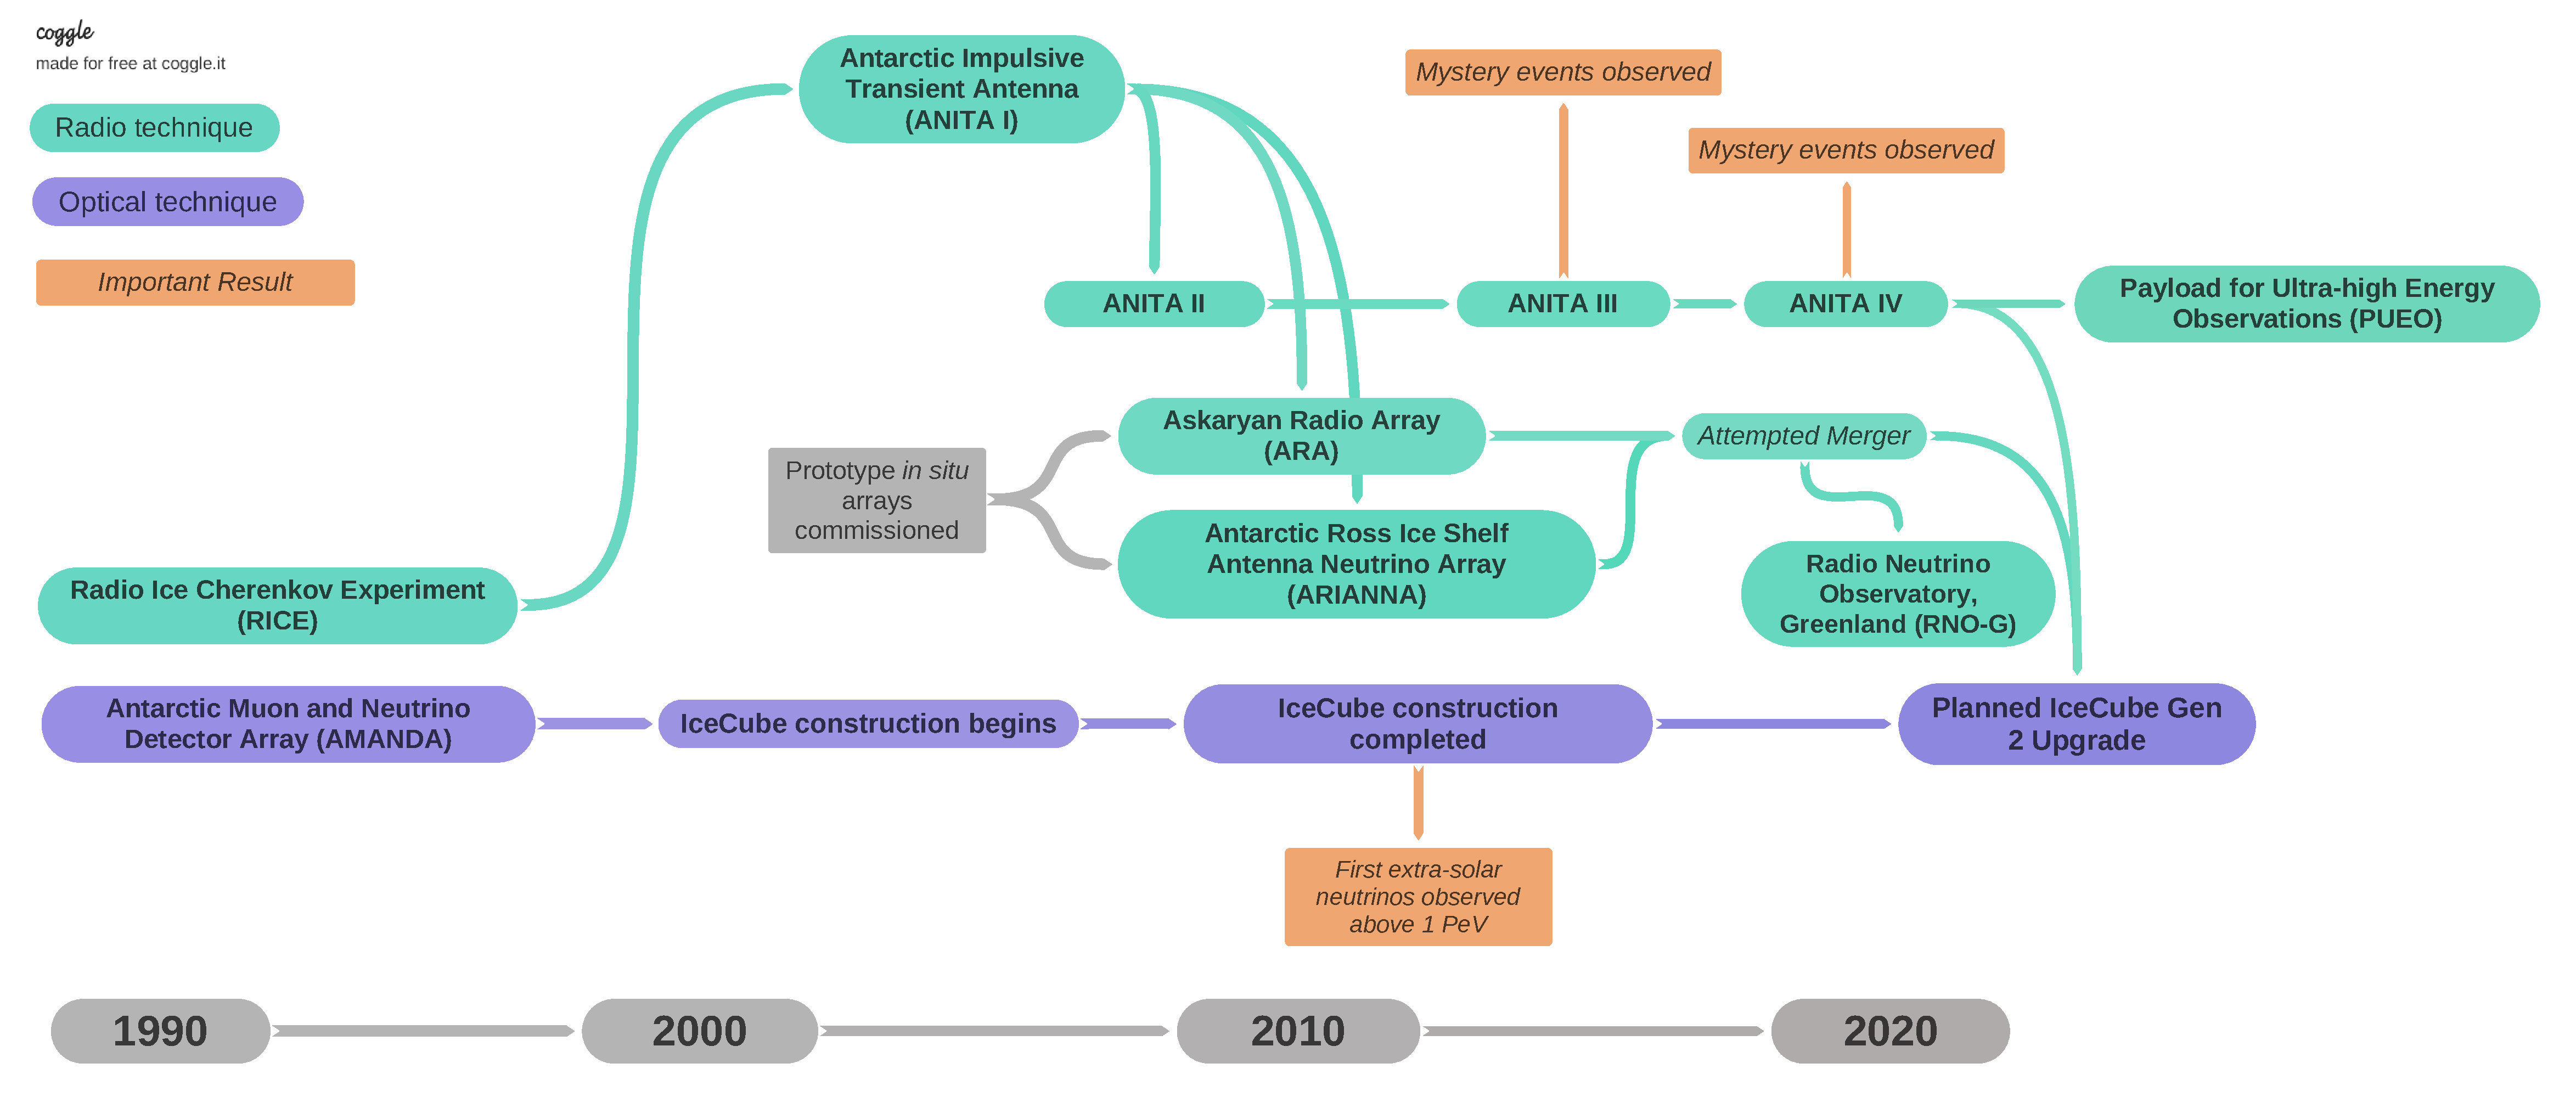
\includegraphics[width=\textwidth]{figures/timeline.pdf}
\caption{\label{fig:flow} A general timeline of the UHE-$\nu$ sub-field of physics.}
\end{figure}

In Sec. \ref{sec:origin}, I reflected on my academic origin story and the contributions I have made to the field.  The plot of that story has taken an interesting and favorable turn for Whittier College.  Not only has the IceCube Collaboration finally recognized the necessity of radio-based detectors \cite{PhysRevD.98.062003}, but IceCube Gen2 designs now include specific designs inspired by ARIANNA.  Further, Whittier College has been invited to become a member institution of The IceCube Collaboration through my scholarship.  This will give us a seat at the table for cutting edge physics research.  I provide a complete list of advantages in Sec. \ref{sec:invite} below.
\\
\vspace{0.25cm}
The diagram in Fig. \ref{fig:flow} illustrates the progress my field has made in the last decade.  IceCube is the largest neutrino detector in the world, and one of the more expensive physics projects in US history (\$0.28 billion).  In perspective, the Mars rover Curiosity cost \$2.5 billion, and the Advanced LIGO gravity-wave detector cost \$1.1 billion.  IceCube was built from a predecessor called AMANDA, constructed at the South Pole for the ice quality and several-kilometer depth\footnote{Being at the South Pole is like being atop a 2.8 km ice mountain.  The ice thickness is needed to form the largest block of ice possible for the detector.}.  AMANDA and IceCube have relied on the \textit{optical technique}, observing tracks of optical photons left by passing neutrinos.  The optical technique requires \textit{digital optical modules} (DOMs) to be deployed 1 kilometer below the surface, separated by 100 meters.  Practically, this limits the detector volume to 1 km$^3$.  After 20 years of detecting neutrinos that originate from cosmic rays striking the atmosphere, IceCube announced the observation of \textit{extra-solar}\footnote{Originating from outside the solar system.} neutrinos with energies of $10^{15}$ electron-volts in 2013 \cite{PhysRevLett.111.021103}.
\\
\vspace{0.25cm}
This result broke the world record for highest-energy neutrino ever observed by humans.  There is also nothing in our solar system capable of accelerating particles to those energies, so the neutrinos at least had to come from outside the solar system.  Currently, IceCube has established a flux of neutrinos below $10^{15}$ electron-volts, and the arrival directions indicate they might have \textit{extra-galactic} origin.  Meanwhile, with the deployment of AMANDA came RICE, the earliest \textit{in situ} Askaryan-class detector.  Deployed before IceCube construction began, RICE operated for just over a decade.
\\
\vspace{0.25cm}
In many ways, RICE was ahead of its time.  Gurgen Askaryan predicted what we call the Askaryan effect in the 1960s.  The radio pulses from neutrinos and other high-energy particles would be conveniently observable as radio pulses, but physicists did not take advantage of this until the 1990s.  In the interim, the Askaryan effect was observed in the lab \cite{PhysRevLett.86.2802} \cite{PhysRevLett.99.171101}. RICE eliminated many of the earlier optimistic models for UHE-$\nu$ sources, and concluded in 2012 with its last publication \cite{PhysRevD.85.062004}.  The time came to build a UHE-$\nu$ detector capable of listening for signals from more ice.  A brilliant idea was hatched: the detector could fly above Antarctica, observing all the ice at once.  Thus, ANITA was born.
\\
\vspace{0.25cm}
ANITA was a UHE-$\nu$ version of the long tradition of cosmic ray balloon flights.  In fact, cosmic rays were originally discovered by Victor Hess and Domenico Pacini in 1911, and Hess used a high-altitude balloon to make observations.  ANITA eventually did observe cosmic rays (which create radio pulses in the atmosphere), along with \textit{the mystery events.}  These mystery events are so-named because they look like cosmic ray signals, but coming up from the ice.  Normally, they would be ideal UHE-$\nu$ signals, but neutrinos with energies above $10^{16}$ electron-volts do not penetrate through the Earth at the observed angles.  Either fundamental physics is wrong, or the interpretation of the signals is.  ANITA has flown four times, and the planned upgrade is called PUEO.
\\
\vspace{0.25cm}
The main drawback with ANITA is that the balloon has to fly 20 km in the air (like a weather balloon).  That means the radio pulse from the UHE-$\nu$ has to travel that much farther to the detector, and the amplitude diminishes.  If the UHE-$\nu$ is extra-energetic, it makes an extra-large radio pulse which can be detected by ANITA.  However, the higher the energy, the rarer the UHE-$\nu$.  Thus, ANITA has not observed the flux observed by IceCube, because the average neutrino in the flux has less than 1\% of the energy necessary to trigger ANITA.  The physics community decided to install two versions of ANITA \textit{in situ} (in the ice), in order to be closer to potential UHE-$\nu$ signals: ARA and ARIANNA.
\\
\vspace{0.25cm}
ARA and ARIANNA had to overcome a number of technical challenges.  While a weather balloon is a standard piece of technology operated by NASA, deploying a physics experiment in the middle of Antarctica is as complex as deploying a satellite orbiting the planet.  Power, communications, data collection, and deployment missions are all technically challenging.  ARIANNA was deployed at Moore's Bay on the Ross Ice Shelf to take advantage of the ocean beneath the ice.  The ocean reflects radio pulses, and thus gives detectors multiple chances to detect them.  ARA was deployed at the South Pole to take advantage of the colder ice.  Colder ice is more radio transparent.  The competition to successfully develop a prototype array lead to seven ARIANNA stations in Moore's Bay, and later two at the South Pole.  ARA deployed three stations at the South Pole, and data from two of them was published.  Later, a fifth\footnote{I never learned from my ARA colleagues what happened to the fourth ARA station.} ARA station was deployed at the South Pole with a \textit{phased array antenna} (see Sec. \ref{sec:neutrino}).
\\
\vspace{0.25cm}
ARA and ARIANNA can detect UHE-$\nu$ with energies of $10^{16}$ electron-volts, \textit{just above} the most energetic portion of the IceCube data.  We are tantalizingly close to breaking the world record for the highest energy neutrino observed, and opening a new window into physics and astrophysics.  The National Science Foundation (NSF) will no longer fund ARA and ARIANNA separately.  In 2018, the two collaborations were tasked with merging and to produce a final detector design at Ohio State University.  The primary issue was the deployment strategy: the ARIANNA design utilizes solar power, RF antennas in the surface snow (called the \textit{firn}), and satellite communications.  The approach is simple and conservative, and hardened for deployment in a harsh environment.  The ARA design calls for drilling boreholes in the ice, similar to IceCube, so that the antennas can be lowered to depths below the \textit{firn}.  The ARA design also involved fiber optics, line-of-sight WiFi, and more antenna channels.  The added complexity leads to a more sensitive experiment, but comes with higher risk.
\\
\vspace{0.25cm}
The merger would have lead to approximately \$250k in funding to Whittier College to work on antenna testing and fabrication.  Unfortunately, the merger also required baby-boomers to compromise.  Since that is impossible, the merger failed.  Meanwhile, European physics foundations decided to fund RNO-G, a hybrid of mostly ARA and some ARIANNA designs to be deployed in Greenland.  Thus, many from ARA floated over to RNO-G.  Greenland can be accessed in the summer of the northern hemisphere, whereas access to Antarctica in general takes place during the northern winter (when the sun is up in Antarctica).  Despite the pandemic, there is an ongoing mission to build the first RNO-G stations.  Meanwhile, the IceCube Collaboration has adopted radio \textit{in situ} arrays as a key design component into the next major upgrade, IceCube Gen2.  Many in our field consider IceCube Gen2 inevitable once the pandemic lifts.  \textit{Whittier College has been invited to become a member institution (see Sec. \ref{sec:invite}).}  Although this comes with no cost to Whittier College, it provides invaluable access to one of the most dynamic physics collaborations in history.  Once complete, IceCube Gen2 will begin to detect the most powerful neutrino events in human history.

\end{document}
